\documentclass[12pt]{article}

\usepackage{color}
%\input{rgb}
%----------Packages----------
\usepackage{amsmath}
\usepackage{amssymb}
\usepackage{amsthm}
\usepackage{amsrefs}
\usepackage{dsfont}
\usepackage{enumerate}
\usepackage{hyperref}
\usepackage{mathrsfs}
\usepackage{stmaryrd}
\usepackage{tikz}
	\usetikzlibrary{matrix}
\usepackage[all]{xy}
\usepackage[mathcal]{eucal}
\usepackage{verbatim}  %%includes comment environment
\usepackage{fullpage}  %%smaller margins
%----------Commands----------

%%penalizes orphans
\clubpenalty=9999
\widowpenalty=9999


%% blackboard bold math capitals
\newcommand{\bbA}{\mathbb{A}}
\newcommand{\bbB}{\mathbb{B}}
\newcommand{\bbC}{\mathbb{C}}
\newcommand{\bbD}{\mathbb{D}}
\newcommand{\bbE}{\mathbb{E}}
\newcommand{\bbF}{\mathbb{F}}
\newcommand{\bbG}{\mathbb{G}}
\newcommand{\bbH}{\mathbb{H}}
\newcommand{\bbI}{\mathbb{I}}
\newcommand{\bbJ}{\mathbb{J}}
\newcommand{\bbK}{\mathbb{K}}
\newcommand{\bbL}{\mathbb{L}}
\newcommand{\bbM}{\mathbb{M}}
\newcommand{\bbN}{\mathbb{N}}
\newcommand{\bbO}{\mathbb{O}}
\newcommand{\bbP}{\mathbb{P}}
\newcommand{\bbQ}{\mathbb{Q}}
\newcommand{\bbR}{\mathbb{R}}
\newcommand{\bbS}{\mathbb{S}}
\newcommand{\bbT}{\mathbb{T}}
\newcommand{\bbU}{\mathbb{U}}
\newcommand{\bbV}{\mathbb{V}}
\newcommand{\bbW}{\mathbb{W}}
\newcommand{\bbX}{\mathbb{X}}
\newcommand{\bbY}{\mathbb{Y}}
\newcommand{\bbZ}{\mathbb{Z}}


\renewcommand{\phi}{\varphi}

\renewcommand{\emptyset}{\O}

\providecommand{\abs}[1]{\lvert #1 \rvert}
\providecommand{\norm}[1]{\lVert #1 \rVert}


\providecommand{\ar}{\rightarrow}
\providecommand{\arr}{\longrightarrow}

\renewcommand{\_}[1]{\underline{ #1 }}


\DeclareMathOperator{\ext}{ext}



%----------Theorems----------

\newtheorem{theorem}{Theorem}[section]
\newtheorem{proposition}[theorem]{Proposition}
\newtheorem{lemma}[theorem]{Lemma}
\newtheorem{corollary}[theorem]{Corollary}


\newtheorem{axiom}{Axiom}


\theoremstyle{definition}
\newtheorem{definition}[theorem]{Definition}
\newtheorem{exercise}[theorem]{Exercise}
\newtheorem{example}[theorem]{Example}
\newtheorem{remark}[theorem]{Remark}
\newtheorem{notation}[theorem]{Notation}
\newtheorem{warning}[theorem]{Warning}


\numberwithin{equation}{subsection}


%----------Title-------------


\begin{document}

\begin{center}
{\large MATH/STAT 230S, SCRIPT 1: Principles of Counting} \\ 
\vspace{.2in}  

\end{center}

\section{Principles of Counting}
\begin{definition}
	A \emph{permutation} is an ordered arrangement of a set.
\end{definition}



\begin{example} How many permutations are there of the set $\{a,b,c\}$?

	\begin{proof}[Solution.] 
		We can list the possible arrangements: $$\{a,b,c\}, \{a,c,b\}, \{b,a, c\}, \{b,c,a\}, \{c,a,b\}, \{c,b,a\}$$ So there are 6.\\ 
		Another way to consider this example is as a tree of options. There are 3 choices for the first element in the permutation. Once, the first element is chosen, there are two remaining elements to choose from for the second element in the permutation. Finally, there is only one element left for the third element in the permutation. The total number of permutations is therefore $(3)(2)(1)=6$.
	\end{proof}

\end{example}


\begin{theorem}\label{permutations}
	There are \_{n!} permutations of a set with $n$ elements.
\end{theorem}


\begin{proof}[Proof of Th \ref{permutations}]
%...insert your explanation here.
Given $n$ elements, there are $n$ possible choices for the first option of the permutations, then $n-1$ possible choices for the second option of each of the respective permutations, and so on until only one possible choice remains for the last option of the permutations.
\end{proof}


\begin{definition}
	A \emph{combination} is an unordered selection of a given number of elements from a set.
\end{definition}

\begin{example} 
	How many combinations of size 3 can be made from the set $\{a,b,c,d\}$?
	\begin{proof}[Solution.]
		In any combination of size 3, exactly one of the elements of the set must be left out. There are 4 elements that could be left out of the set. So, their are 4 combinations of size 3. Another way to say this is ${ 4\choose 3}=4$.
	\end{proof}
\end{example}

\begin{notation}
	The notation ${ n\choose k}$ is read as ``$n$ choose $k$."\\ ${ n\choose k}$ is equal to the number of ways to select $k$ objects from a set of $n$ objects (without consideration for the order of the selection).
\end{notation}

\begin{theorem}\label{combination}
	${n \choose k}=\dfrac{n!}{k! (n-k)!}$
\end{theorem}

\begin{proof}[Proof of Th \ref{combination}]
%insert your explanation here.
Given $n$ elements, the total number of permutations of length $k$ will be: \\
\[n\cdot (n-1)\cdots (n-(k-1))=\dfrac{n!}{(n-k!)}\]
Now, as there are $k!$ number of ways to order $k$ elements, we divide the total number of permutations of length $k$ by $k!$ to get the total number of combinations of length $k$.
\end{proof}

\begin{example}
% Write your own example and solution involving combinations.
Given the Roman senate had 300 senators and 2 consuls elected every year, how many ways could any 2 senators serve together as consuls in a given year?
\begin{proof}[Solution.]
	Given this is a combinations problem where 2 consuls are ``chosen" out of 300 senators or ``300 choose 2", using Theorem 1.7: \\
	\# of consul combinations $={300\choose 2}=\dfrac{300!}{2!(300-2)!}=44850$
\end{proof}
After serving their terms, former consuls can serve as governors in any of the Roman provinces. Given there are 15 provinces and one governor post for each province, how many different ways could two former consuls become provincial governors?
\begin{proof}[Solution.]
	Given this is a permutation problem, we can determine how for the first former consul that there are 15 available governor posts and consequently 14 available governor posts for the second, meaning there are $15\cdot 14 = 210$ total number of provincial governor permutations.
\end{proof}
\end{example}

\begin{theorem}\label{binomial}
(Binomial Theorem) $\displaystyle(x+y)^n=\sum_{k=0}^n {n \choose k}x^ky^{n-k}$
\end{theorem}

\begin{proof}[Proof of Th \ref{binomial}]
    As $n={n\choose 1}={n\choose n-1}$ and likewise ${n\choose k}={n\choose n-k}$
    \begin{align*}
        (x+y)^n=(x+y)\cdot (x+y)\cdots (x+y)=1x^n
            &+{n\choose 1}x^{n-1}y^1+\cdots + \\
            &+{n\choose n - 1}x^1y^{n-1} + 1y^n
    \end{align*}
    Relates to Pascal's triangle for binomial expansion \\
    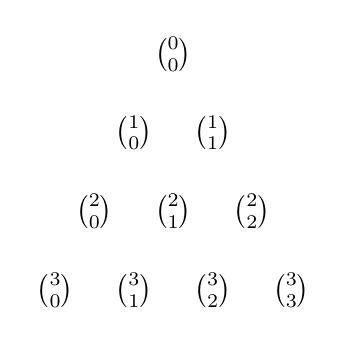
\begin{tikzpicture}
        \foreach \n in {0,...,3} {
          \foreach \k in {0,...,\n} {
            \node at (\k-\n/2,-\n) {$\n\choose \k$};
          }
        }
    \end{tikzpicture}
\end{proof}

\end{document}
